\documentclass{article}

\usepackage{a4wide}
\usepackage[utf8]{inputenc}
\usepackage[T1]{fontenc}
\usepackage[french]{babel}
\usepackage[babel=true]{csquotes} % guillemets français
\usepackage{graphicx}
\graphicspath{{Images/}}
\usepackage{color}
\usepackage{hyperref}
\hypersetup{colorlinks,linkcolor=,urlcolor=blue}

\usepackage{amsmath}
\usepackage{amssymb}


\title{Rapport Slime}
\author{Goomanee Izhaar, Coutin Matthias, Chan Chun Tim Alan}
\date{\today}

\begin{document}

\maketitle % pour écrire le titre


%% Le résumé:
\begin{abstract}

\end{abstract}

\section{Introduction}
\label{section:hello} % pour faire référence à la section ailleurs (\ref{...} voir plus bas)

Dans le cadre du projet Mobile, nous avons réfléchi un moyen d’exploiter les différentes contraintes exigées par monsieur Etienne PAYET( Changements de configuration, Internationalisation, Géolocalisation, Capteurs, Lecture audio, Gestes courants, Appareil photo). De ce fait après mûre réflexion nous avons pensé à une application basée sur le principe du tamagotchi c’est dire élevé un être ( on a choisi un slime), pour la côté nouvelle technologie nous avons implementer la réalité augmenté. Les contraintes exigées nous ont orientés sur élever un slime avec des efforts physiques car il faut utiliser les capteurs du smartphone. On peut dire que c’est avec effort que l’on élève un slime !

\begin{center}
  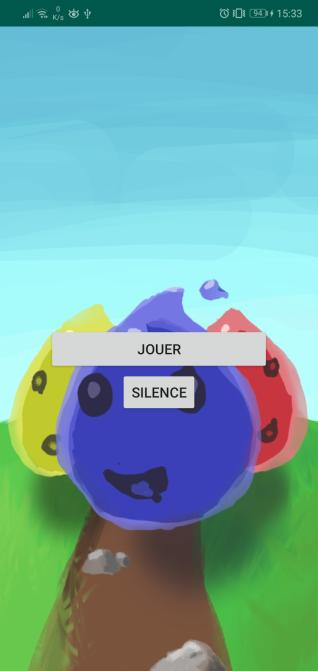
\includegraphics[scale=0.4]{Main.jpg}
\end{center}
\newpage


\section{Le but et le fonctionnement de l'application}
\subsection{Le but de l'application}

Le but de l'application est simple, c'est juste un animal de compagnie que l'on doit s'occuper attentivement, et repondre a ses besoins.

Par exemple, dans notre version, le tamagochi possede 3 besoins :

\begin{itemize}
    \item Vie > on doit porter attention a sa vie, si il n'est pas dans de bonne consitions, sa vie diminuera rapidement
    \item Energy > On doit s'aasurer que l'animal a un minimum temps de repos, dans le cas contraire, il sera très épuisé.
\end{itemize}

\begin{center}
  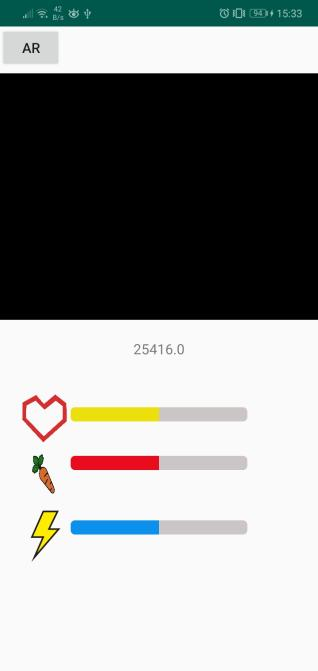
\includegraphics[scale=0.5]{tama.jpg}
\end{center}


\subsection{La description générale du jeu}

Le jeu comprend plusieurs fenêtres différentes. Tout d’abord, vous avez la fenêtre principale sur laquelle vous pouvez lancer le jeu si vous le souhaitez. Une fois lancer, une fenêtre apparaît et le jeu se met en marche, le slime est sur sa position initiale, il peut faire des mouvements si vous le souhaitez en appuyant sur le slime, toutefois pour le repositionner à sa position initiale, il faut appuyer 2 fois sur le slime. Cependant, il ne faut pas oublier de porter attention aux trois critères pour le bon fonctionnement du slime, tels que sa vie, son energy et son humeur, dans le cas contraire, vouz risquerait de perdre votre Tamagotchi.
Ce qui rend le jeu unique, c'est la partie réalité augmentée, il existe un bouton <AR> en haut de l'écran qui vous permetterez d'utiliser votre caméra pour profiter de cette technique et faire apparaitre automatiquement le slime sur un endroit plat.


\newpage
Voici les différentes classes et activités Java utilisés en\textbf{Android}:
\begin{itemize}

\medskip
\item MainActivity > Page principale
\item GameActivty > Lance le jeu
\item ArActivity > La réalité augmenté
\item GameView > Contient tout les codes et les méthodes du jeu
\end{itemize}
% \cite{...} permet de faire référence à des éléments de la
% bibliographie.

\medskip

Voici les différentes classes Swift sur \textbf{IOS}:
\medskip


\section{Architecture du code}

Contrairement à la section 2, on va détailler les codes en plus approfondis On va commencer tout d’abord par Android, en décrivant dans l’ordre de l’execution. Puis par la suite, on aura la section iOS

\subsection{Android}

\begin{verbatim}
// Musique 

MediaPlayer mp;

....

protected void onCreate(Bundle savedInstanceState) {
    ....
    if(silence) {
            mp = MediaPlayer.create(this, R.raw.gamemus);

            mp.setLooping(true);
            mp.start();
        }
    ....
}

// Geolocalisation 

package com.androdocs.currentlocation;

import androidx.appcompat.app.AppCompatActivity;
import androidx.core.app.ActivityCompat;
import android.Manifest;
import android.content.Context;
import android.content.pm.PackageManager;
import android.location.LocationManager;
import android.os.Bundle;

public class MainActivity extends AppCompatActivity {

    int PERMISSION_ID = 44;

    @Override
    protected void onCreate(Bundle savedInstanceState) {
        super.onCreate(savedInstanceState);
        setContentView(R.layout.activity_main);
    }

    private boolean checkPermissions() {
        if (ActivityCompat.checkSelfPermission(this, Manifest.permission.ACCESS_COARSE_LOCATION) == PackageManager.PERMISSION_GRANTED &&
                ActivityCompat.checkSelfPermission(this, Manifest.permission.ACCESS_FINE_LOCATION) == PackageManager.PERMISSION_GRANTED) {
            return true;
        }
        return false;
    }

    private void requestPermissions() {
        ActivityCompat.requestPermissions(
                this,
                new String[]{Manifest.permission.ACCESS_COARSE_LOCATION, Manifest.permission.ACCESS_FINE_LOCATION},
                PERMISSION_ID
        );
    }

    private boolean isLocationEnabled() {
        LocationManager locationManager = (LocationManager) getSystemService(Context.LOCATION_SERVICE);
        return locationManager.isProviderEnabled(LocationManager.GPS_PROVIDER) || locationManager.isProviderEnabled(
                LocationManager.NETWORK_PROVIDER
        );
    }

    @Override
    public void onRequestPermissionsResult(int requestCode, String[] permissions, int[] grantResults) {
        super.onRequestPermissionsResult(requestCode, permissions, grantResults);
        if (requestCode == PERMISSION_ID) {
            if (grantResults.length > 0 && grantResults[0] == PackageManager.PERMISSION_GRANTED) {
                // Granted. Start getting the location information
            }
        }
    }
}

// Podometre

private SensorManager sensorManager;
private Sensor sensor;


....

protected void onCreate(Bundle savedInstanceState) {
    ....
    sensorManager = (SensorManager) getSystemService( Context.SENSOR_SERVICE );
    ....
}
....


public void onResume() {

        ....

        sensor = sensorManager.getDefaultSensor( Sensor.TYPE_STEP_COUNTER );

        if (sensor != null) {
            sensorManager.registerListener( this, sensor, SensorManager.SENSOR_DELAY_UI );
        } else {
            //step.setText( "error" );
        }
        ....

}

public void onPause() {
        super.onPause();

        running = false;
        sensorManager.unregisterListener( this );

    }


@Override
    public void onSensorChanged(SensorEvent event) {
        if (running) {
            step.setText( "" + event.values[0] );
        }

    }

// Ar 

    private ArFragment arFragment;
    private ModelRenderable mon_modele;

    @Override
    protected void onCreate(Bundle savedInstanceState) {
        super.onCreate(savedInstanceState);
        setContentView(R.layout.activity_ar);
        arFragment = (ArFragment)getSupportFragmentManager().findFragmentById(R.id.ux_fragment);

        ModelRenderable.builder()
                .setSource(this, Uri.parse("slime.sfb")) // Modèle 3D
                .build()
                .thenAccept(renderable -> mon_modele = renderable);

        arFragment.setOnTapArPlaneListener(
                (HitResult hitResult, Plane plane, MotionEvent motionEvent) -> {
                    if (mon_modele == null) {
                        return;
                    }
                    if (plane.getType() != Plane.Type.HORIZONTAL_UPWARD_FACING) {
                        return;
                    }


                    //On créé le point d'encrage du modèle 3d
                    Anchor anchor = hitResult.createAnchor();
                    AnchorNode anchorNode = new AnchorNode(anchor);
                    anchorNode.setParent(arFragment.getArSceneView().getScene());

                    //On attache ensuite notre modèle au point d'encrage
                    TransformableNode Node = new TransformableNode(arFragment.getTransformationSystem());
                    Node.setParent(anchorNode);
                    Node.setRenderable(mon_modele);
                    Node.select();


                }
        );
    }

\end{verbatim}



\section{Recherche sur le game design }
\subsection{Logiciel Krita}
Avec Krita nous avons dans un premier temps dessiner les premiers modèles du slime.
\begin{center}
  
\includegraphics[scale=0.3]{slime01.png}
\end{center}


\section{Création du slime sur Blender}
\subsection{Le Slime}
\begin{center}
  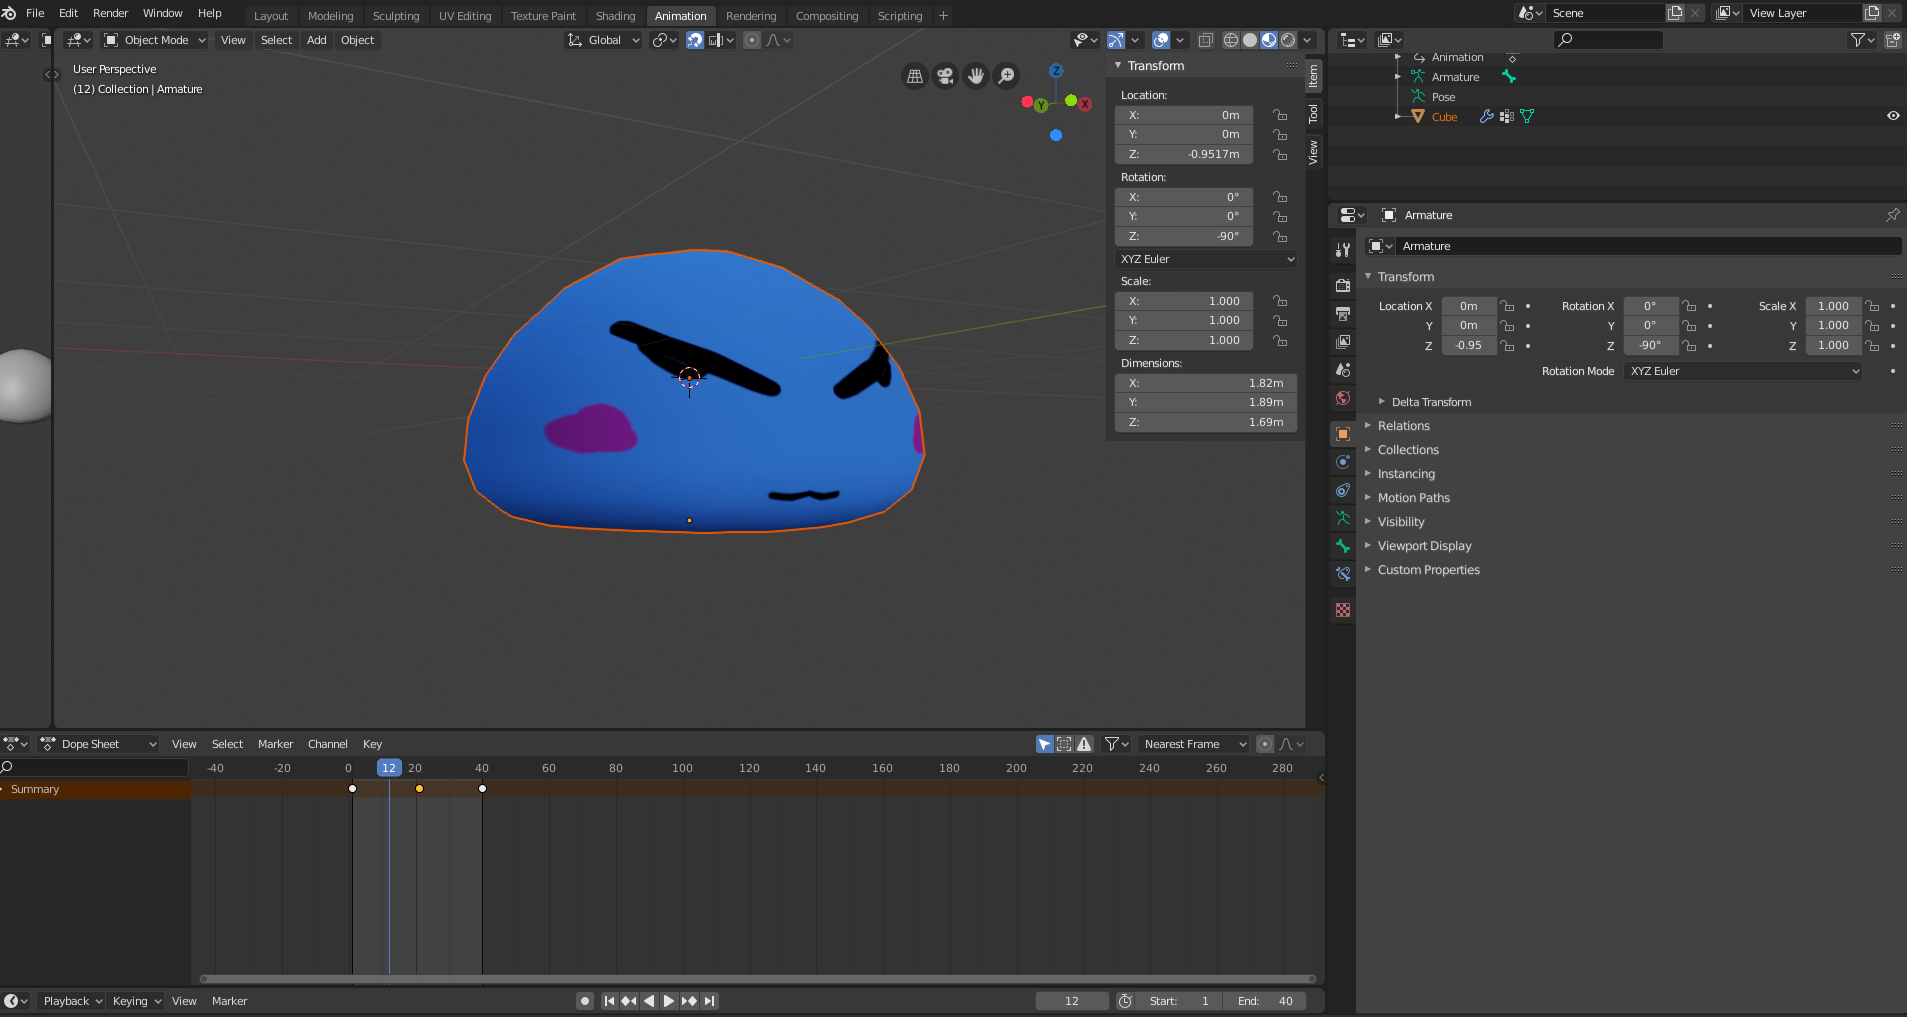
\includegraphics[scale=0.2]{blender.png}
\end{center}
\subsection{Squelette du slime}
Le squelette nous permet d'avoir une animation pour le slime.
\begin{center}
  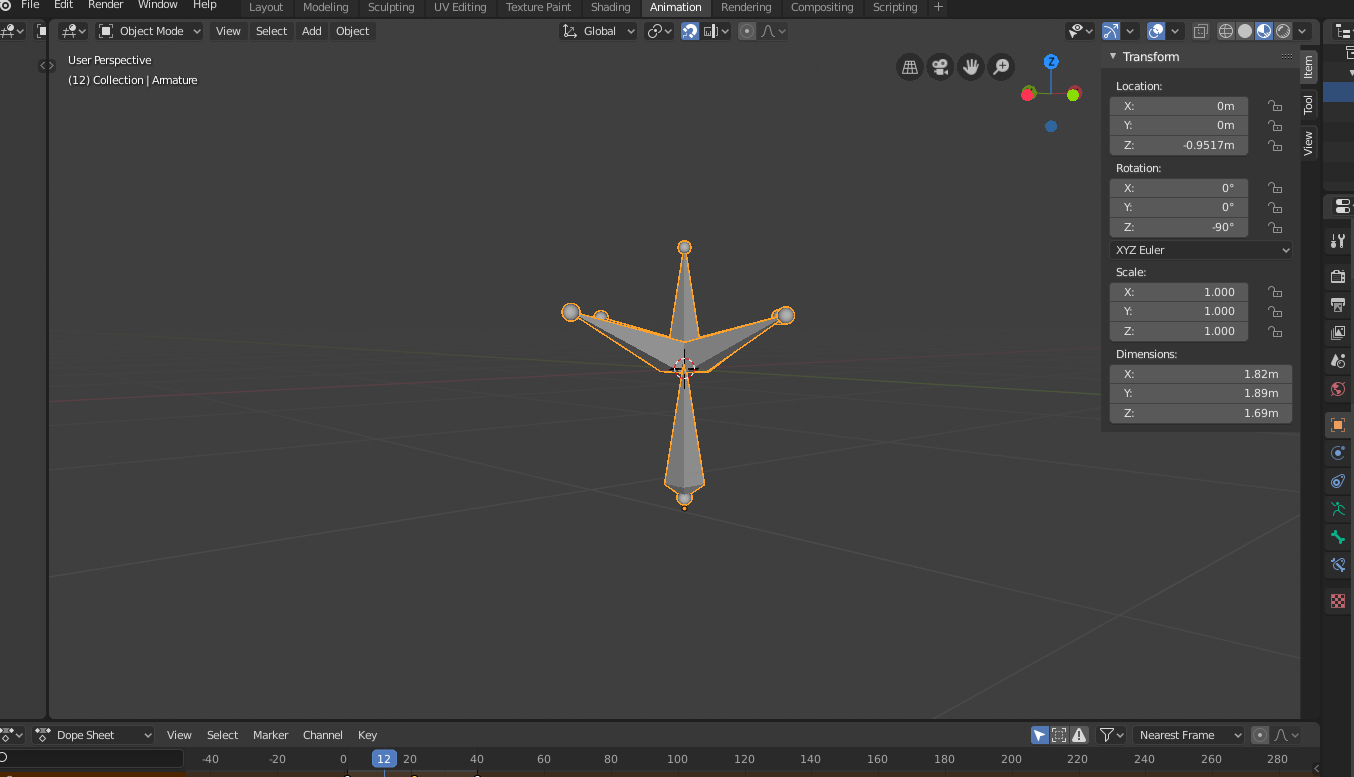
\includegraphics[scale=0.3]{squeletteSlime.png}
\end{center}
\newpage
\section{Création du model 3D sous RealityKit}
\subsection{RealityComponent}
Avec cette interface graphique Apple nous ont offert un moyen très simple d'implementer des objets graphiques 3D sous swift. 
\begin{itemize}
    \item Point d'ancrage > permet de détecter une surface pour ajouter le modèle 3D
    \item Comportement > permet de créé des animations pour votre modèle 3D (nous avons créé le nôtre sur Blender, il est possible de l'utiliser avec des fichiers 3D en .usdz)
    \item La texture  > La texture est créé sous le logiciel Krita 
    \item Ensuite il suffit d'exporter le fichier sous XCode 
\end{itemize}
\begin{center}
  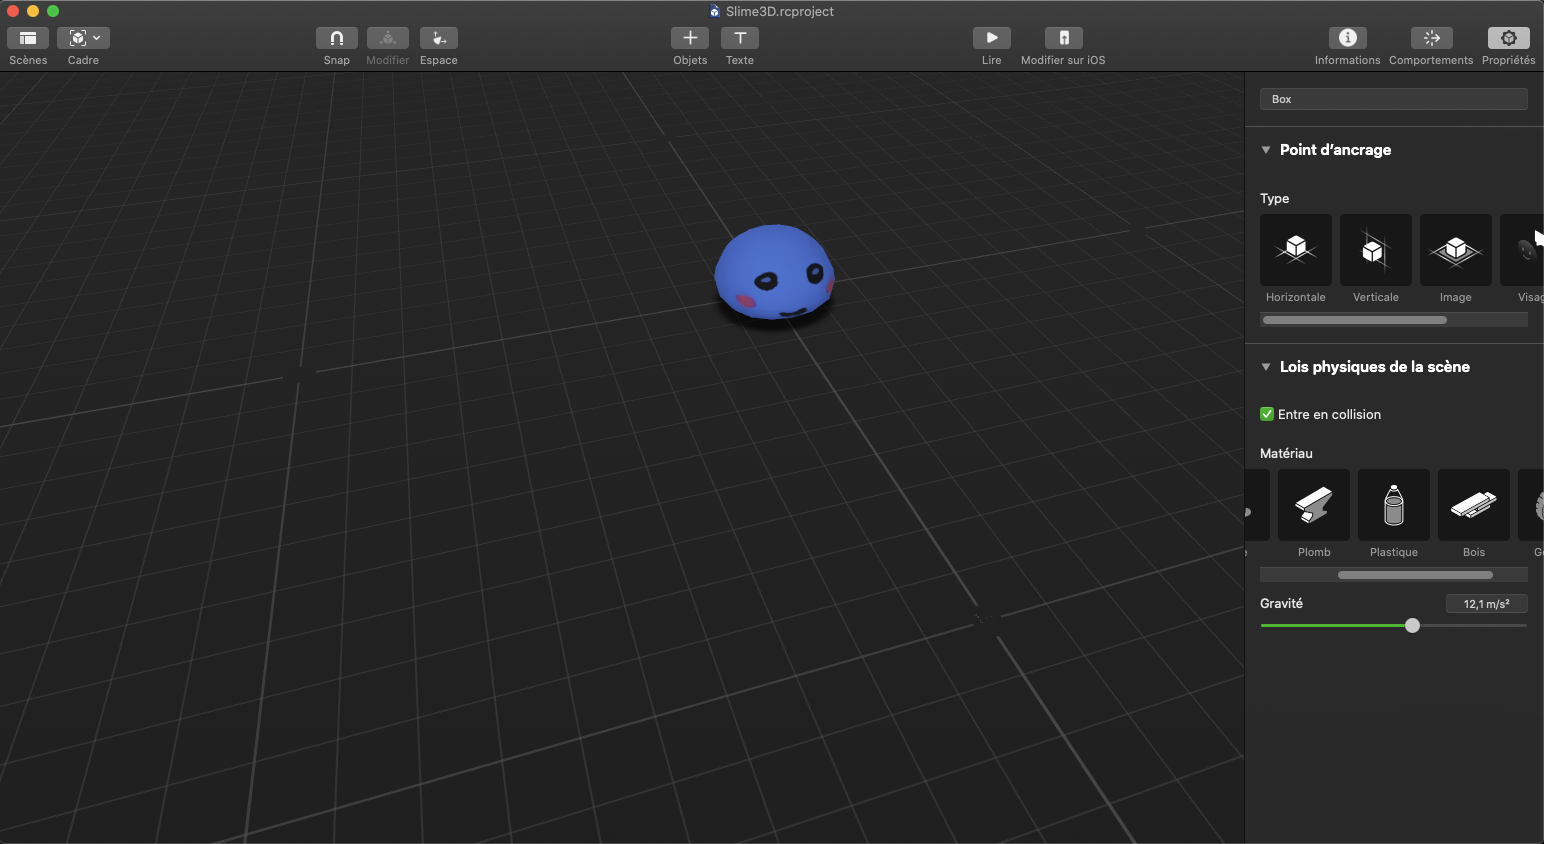
\includegraphics[scale=0.3]{realitycompo.png}
\end{center}


\subsection{Création du jeux IOS}
\subsection{Model sous IOS }
\begin{center}
  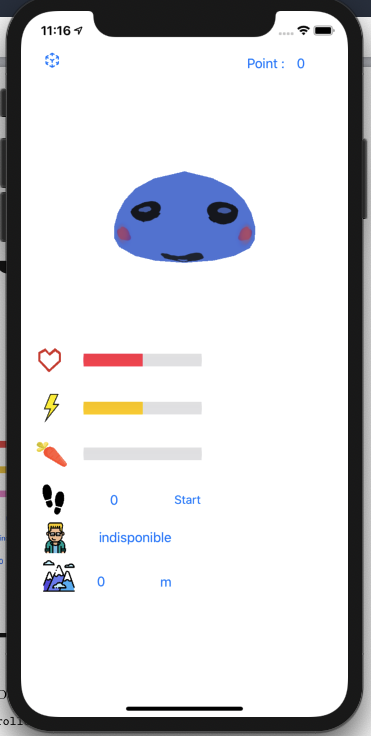
\includegraphics[scale=0.4]{iphone02.png}
\end{center}
\subsection{RealityKit}
Code d'implementation du modèle 3D (très simple)
\begin{verbatim}
    class RealityView: UIViewController {

    @IBOutlet weak var arView: ARView!
    var slime : Slime3D.Box!
    override func viewDidLoad() {
        super.viewDidLoad()

        slime = try! Slime3D.loadBox()
        slime.generateCollisionShapes(recursive: true)
        arView.scene.anchors.append(slime)
    }
    
\end{verbatim}
\newpage
\subsection{Podomètre }
fonction du podomètre (je mets pas tout il y a trop)
Récupere les données du podomètre incrémente une variable avec modulo 2 pour les points 
\begin{verbatim}`
private func startCountingSteps() {
            pedometer.startUpdates(from: Date()) {
                [weak self] pedometerData, error in
                guard let pedometerData = pedometerData, error == nil else { return }

                DispatchQueue.main.async {
                    self?.label1.text = pedometerData.numberOfSteps.stringValue
                    self?.popo += (pedometerData.numberOfSteps.intValue) % 2
                    let lolo = String(self?.popo ?? 0)
                    self?.Point.text = lolo
                    
                }
            }
        }

\end{verbatim}
\subsection{Altitude }
Récupere l'atitude grâce à la geolocalisation 
\begin{verbatim}
   func locationManager(_ manager: CLLocationManager, didUpdateLocations locations: [CLLocation]) {
        let location  = locations[0]

        label3.text = String(Int(location.altitude))
    }
\end{verbatim}
\section{Conclusion}
 français
Pour conclure le projet que nous avons effectué, nous a permis de pouvoir mettre en pratique des techniques vues en cours telles que la géolocalisation et l’utilisation d'autres fonctionnalités liées à Android et IOS. Nous avons pu aussi aborder des technologies qu’on ne maitrise pas au début comme la réalité augmentée, nous avons dû nous documenter et faire un travail de recherche. Ce projet nous a permis aussi d’avoir un peu plus expérience sur le travail en groupe et l’organisation. En d'autres termes malgré quelque difficulté nous avons pu expérimenter dans une certaine mesure, la mise en oeuvre d’un véritable projet avec les problèmes qui si attaches.

%%% La bibliographie:
\bibliographystyle{plain}
\bibliography{ma_biblio}

\end{document}
